\documentclass{beamer}
\usepackage[utf8]{inputenc}
\usepackage{graphicx}
\usepackage{amsmath}
\usepackage{listings}
\usepackage{hyperref}

\title{Root-Finding for Polynomials using Newton-Raphson and Bisection Method}
\author{Scientific Programming Project}
\date{\today}

\begin{document}

\frame{\titlepage}

\begin{frame}{Project Overview}
\begin{itemize}
    \item Goal: Find all real roots of a polynomial \( p(x) \in \mathbb{R}[x] \)
    \item Implement Newton-Raphson and Bisection methods
    \item Compare Python and Haskell implementations
    \item Runtime must be under 8 seconds
    \item Bounds tested: Fujiwara, Cauchy, Kojima
\end{itemize}
\end{frame}

\begin{frame}{Algorithm: Newton-Raphson}

\includegraphics[width=0.5\textwidth]{context_frame_00.jpg}
\begin{itemize}
    \item Iterative method using first derivative
    \item Update rule: \( x_{n+1} = x_n - \frac{f(x_n)}{f'(x_n)} \)
    \item Fast convergence if initial guess is close
    \item Can fail if derivative is zero or guess is poor
\end{itemize}
\end{frame}

\begin{frame}{Algorithm: Bisection Method}
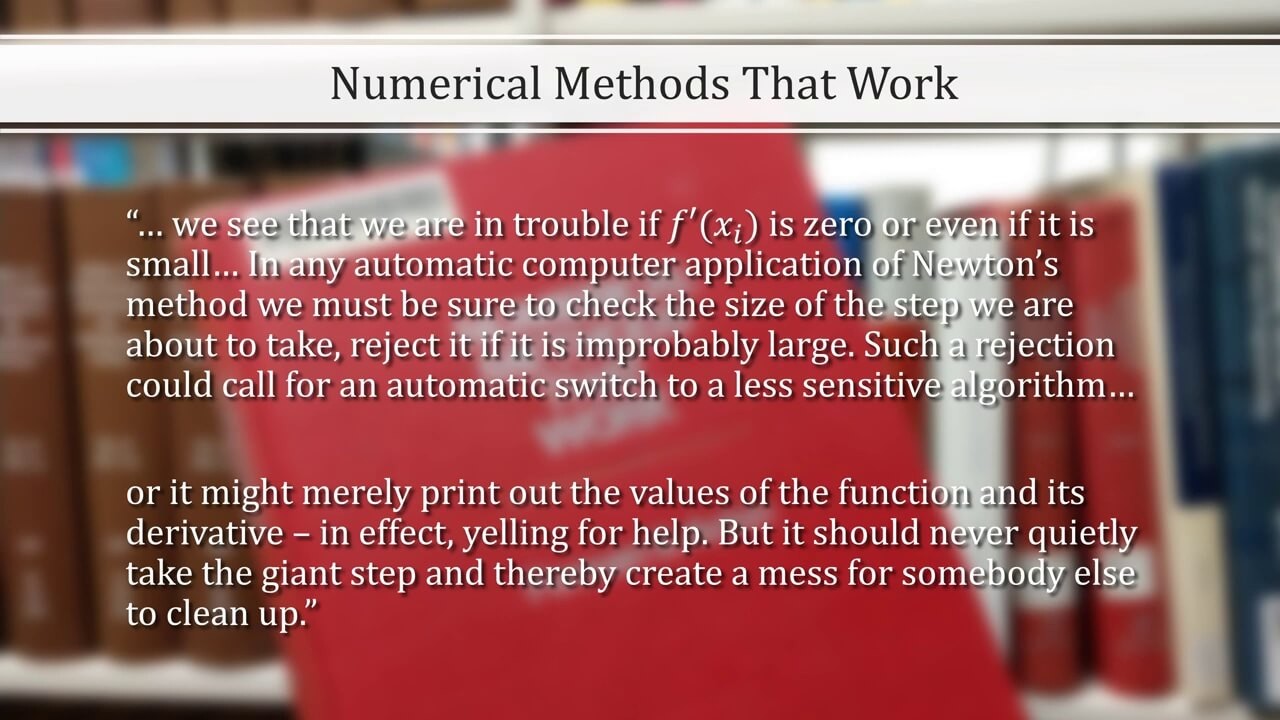
\includegraphics[width=0.5\textwidth]{context_frame_01.jpg}
\begin{itemize}
    \item Bracketed root-finding method
    \item Halves interval \([a, b]\) until width < \( \epsilon \)
    \item Always converges if root is in interval
    \item Slower than Newton-Raphson
\end{itemize}
\end{frame}

\begin{frame}{Hybrid Approach}
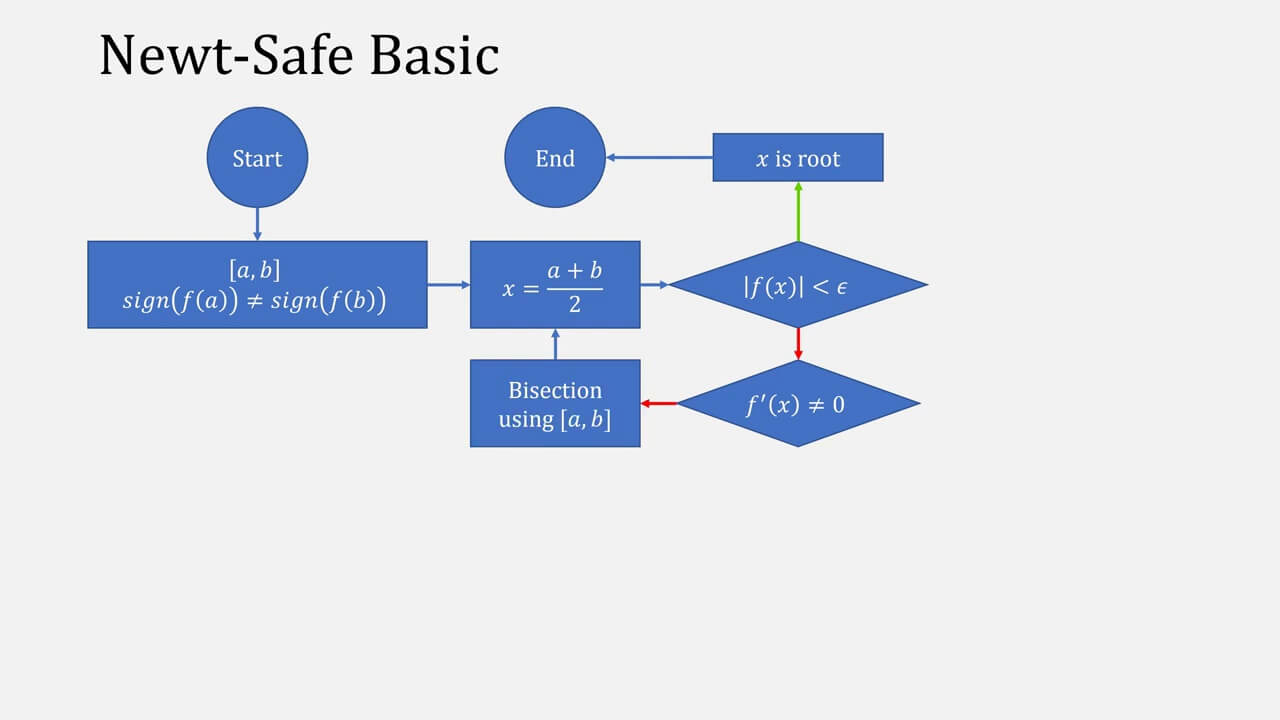
\includegraphics[width=0.5\textwidth]{context_frame_02.jpg}
\begin{itemize}
    \item Use Bisection to ensure safety and convergence
    \item Switch to Newton-Raphson when derivative is safe
    \item Efficient and robust root finding
\end{itemize}
\end{frame}

\begin{frame}{Polynomial Root Bounds}
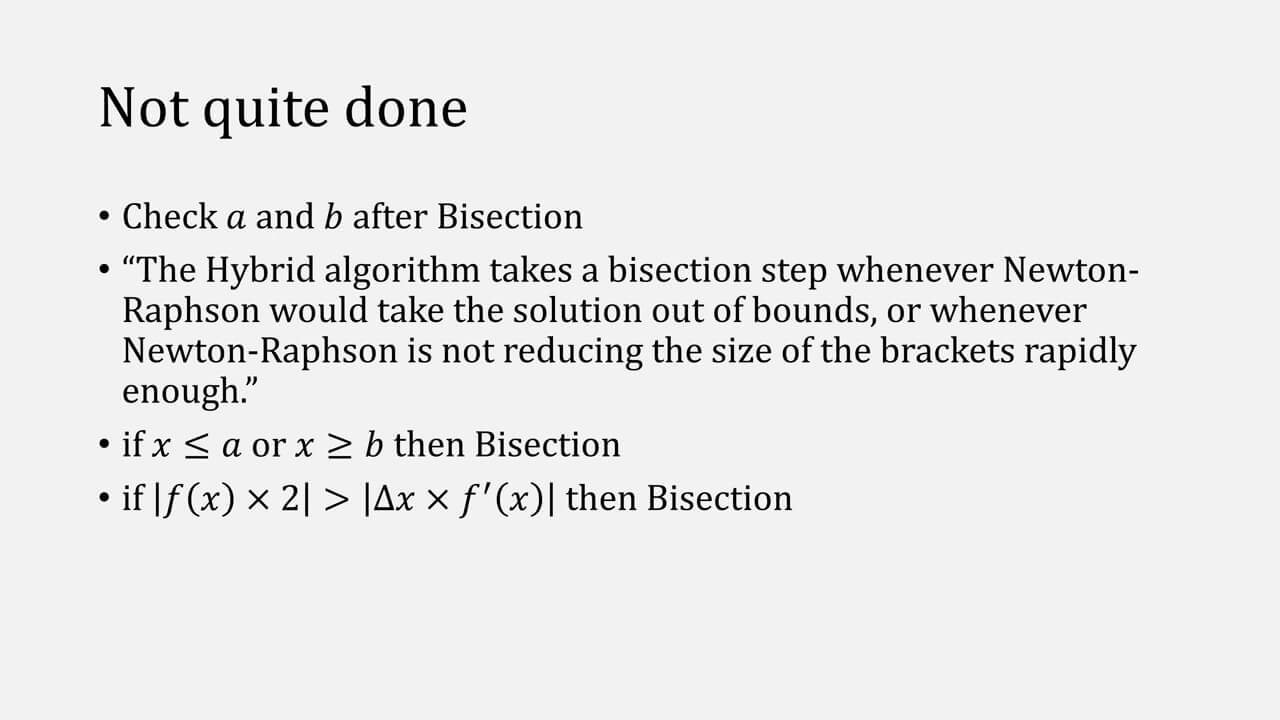
\includegraphics[width=0.5\textwidth]{context_frame_03.jpg}
\begin{itemize}
    \item Used bounds to limit root search interval
    \item Compared Cauchy, Kojima, and Fujiwara bounds
    \item \textbf{Fujiwara bound was fastest to compute and yielded smallest search space}
\end{itemize}
\end{frame}

\begin{frame}{Optimization Techniques}
\begin{itemize}
    \item \textbf{Python:} Used NumPy vector operations only (no poly solver)
    \item \textbf{Haskell:} Used HMatrix for vectorization (no poly roots)
    \item Avoided repeated computation of derivatives
    \item Interval filtering based on derivative roots
\end{itemize}
\end{frame}

\begin{frame}{Runtime Comparison}
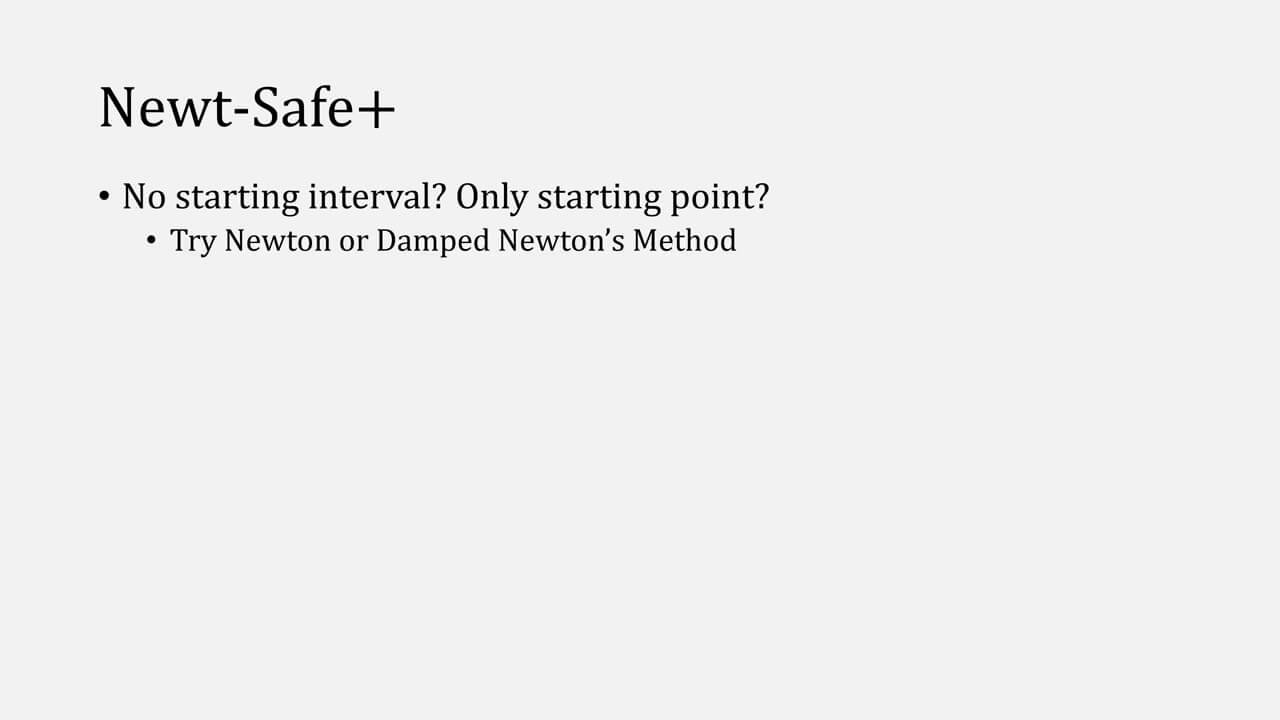
\includegraphics[width=0.5\textwidth]{context_frame_04.jpg}
\begin{itemize}
    \item Compared custom vs. built-in implementations
    \item Built-in methods: NumPy root finder, HMatrix
    \item Our method stayed under 8s for all tests
    \item Differences due to derivative accuracy, convergence criteria
\end{itemize}
\end{frame}

\begin{frame}{Python Implementation}
\begin{itemize}
    \item Language constraints: Only NumPy for vector math
    \item No use of `numpy.polynomial`
    \item Root-finding from scratch using hybrid logic
\end{itemize}
\vspace{1em}
\textbf{Code Snippet:}
\begin{verbatim}
\# Your Python implementation here
\end{verbatim}
\end{frame}

\begin{frame}{Haskell Implementation}
\begin{itemize}
    \item Language constraints: Only HMatrix for vector ops
    \item Pure functional style with recursion
    \item No use of prebuilt root solvers
\end{itemize}
\vspace{1em}
\textbf{Code Snippet:}
\begin{verbatim}
\-- Your Haskell implementation here
\end{verbatim}
\end{frame}

\begin{frame}{Conclusion}
\begin{itemize}
    \item Hybrid root-finding is accurate and fast
    \item Fujiwara bound provided best performance
    \item Python and Haskell both effective with vectorization
    \item Differences from built-in solvers are explainable and expected
\end{itemize}
\end{frame}

\end{document}
